\documentclass[12pt]{article}

% ============
% | Preamble |
% ============

    % Package Imports
        \usepackage[bottom]{footmisc}  % Force footnotes to the bottom of page.
        \usepackage[margin=2cm]{geometry}
        \usepackage[nottoc,numbib]{tocbibind}
        \usepackage[T1]{fontenc}  % Set encoding to correct ASCII.
        \usepackage{blindtext}
        \usepackage{float}  % Force image insertion position.
        \usepackage{graphicx}  % Allow image insertion.
        \usepackage{hyperref}  % Use URLs (for bibliography).
        \usepackage{minted}  % Provide syntax highlighting for code snippets.
        \usepackage{pdftexcmds}
        \usepackage{titlesec}

    % Other Stuff
        \graphicspath{ {media/} } % Specify path to content.

        \newcommand{\HRule}{\rule{\linewidth}{.5mm}} % Draw lines for title page.
        \newcommand{\sectionbreak}{\clearpage} % Define new pages after sections (Broken)?

% ================
% | End Preamble |
% ================

% ===========
% | Content |
% ===========

\begin{document}
    \begin{titlepage}
    \vspace*{1cm}
    \begin{center}

        \textsc{\LARGE University of Queensland}\\[1.5cm]

        \textsc{\Large COSC3000 Semester 1 2015}\\[0.5cm]

        % Title
        \HRule \\[0.4cm]
        { \huge{ \bfseries Model UQ}\\ Computer Graphics Report \\[0.4cm] }
        \HRule \\[0.5cm]

        \vspace*{5mm}
        \textsc{\Large Thomas Cranny}\\[0.5cm]
        42920368
        \vspace*{1cm}

        \begin{abstract}
            \texttt{TODO}
        \end{abstract}

        \vfill
        % Bottom of the page
        {\large \today}

    \end{center}
\end{titlepage}
% End title Page.

\tableofcontents
    \section{Introduction} % (fold)
\label{sec:introduction}
    % Set up introduction.
    The aim of the project was to construct a viable 3D visual representation of the University of Queensland's St Lucia campus.
    The rationale for undertaking this project was multifaceted; it is a thematic continuation of the previous data visualisation project, and it serves as a useful and relevant application of computer graphics techniques.\\

    % What:
    Following the initial proposal, the end goal of the project was to create a visually recognisable recreation of the UQ St Lucia campus.
    In order to accomplish this, multiple computer graphics techniques were utilised to produce the end result.\\

    % Why:
    The previous data visualisation project aimed to analyse the relationships between the faculties, courses, majors, and programs offered by UQ.
    This project is a continuation of the UQ centric theme, however not much else is continued through into this project.

    The rationale of visualising the St Lucia campus in a three dimensional model is to provide a better method of gaining a spatial awareness of the campus' layout and structures.
    This stems from recalling the unhelpfulness of most UQ maps when trying to navigate the campus for the first time.
    Due to the odd shapes of many buildings, the presence of many annexes and similarly labelled and named buildings, the ambiguity between roads, walkways, and viable pathways, and the dense arrangement of buildings, sufficiently learning the layout of the campus may even take weeks.

    \begin{figure}[H]
        \centering
        \fbox{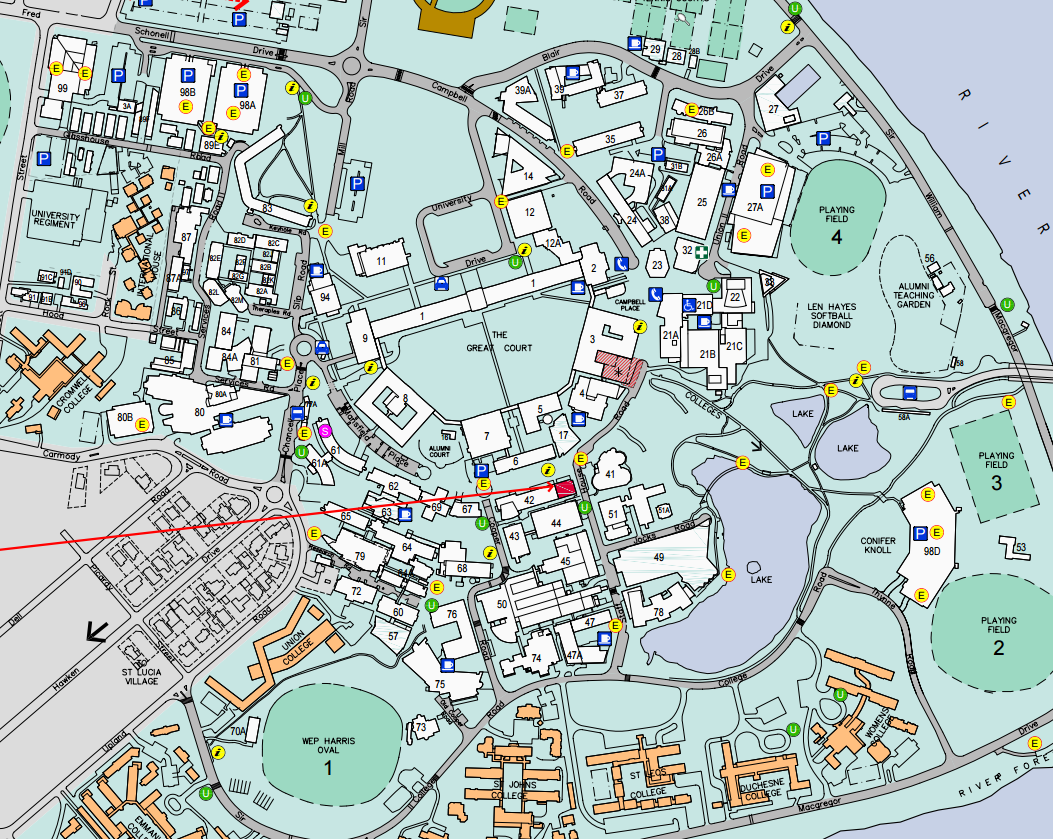
\includegraphics[width=0.75\textwidth]{map}}
        \caption{
            Official University of Queensland St Lucia map \cite{uq_map}. Note the densely packed, oddly shaped and often conjoined layout of the buildings.
        }
        \label{fig:uq_flat_map}
    \end{figure}

    Static maps, such as in Figure \ref{fig:uq_flat_map}, can have high technical accuracy, but are often convoluted and typically don't convey a good physical model of an environment to a reader.
    Abstract two dimensional maps typically require a lot of cross checking between the map and the physical surroundings, in order to correlate real landmarks with what the map displays.
    If structures and landmarks could be better represented to correlate with their real life counterparts more realistically, users will be able to visualise and integrate a locale much more quickly and effectively than attempting to correlate an abstract diagram to their surroundings.


% section introduction (end)

    \section{Methods} % (fold)
\label{sec:methods}

    \subsection{Technical Overview} % (fold)
    \label{sub:technical_overview}
        The project was implemented using the graphics capabilities of modern browsers, primarily through the three.js JavaScript library, and GLSL shaders.
        The main features incorporated include:
        \begin{itemize}
            \item Mouse interactivity.
            \item Texture and bump mapping.
            \item Dynamic model creation.
            \item Lighting and shadow casting.
            \item Animation.
            \item Constructive geometry.
            \item GLSL shaders.
        \end{itemize}
    % subsection technical_overview (end)

    \subsection{Graphics Environment: WebGL and Three.js} % (fold)
    \label{sub:graphics_environment_webgl_and_three_js}
        The project was done using WebGL, an implementation of the OpenGL specification used with in modern web browsers.
        WebGL is designed as a rendering context for the HTML Canvas element \cite{khronos_webgl}.
        The rationale for using WebGL was based around the portability of web pages, and the ubiquity of web browsers.
        Equivalent OpenGL projects written in C have more complex and fragile requirements, such as a compilers, library headers, and platform specific binaries; and Python requires similar dependencies and suffers reduced performance in addition.\\

        In order to access the browsers rendering capabilities, the \textit{three.js} JavaScript library was used, as it is well documented, and has an extensive corpus of examples online.
        It provides a programming environment well suited for graphics programming in JavaScript.
        While JavaScript is more object orientated than the venerable C bindings for OpenGL, it maintains a close equivalence to native GL instructions, with a cleaned up API and astute use of flexible JavaScript objects\footnote{`\textit{JSON}' is also often used, it stands for JavaScript Object Notation, and is a useful data serialisation format}.
    % subsection graphics_environment_webgl_and_three_js (end)

    \subsection{Features} % (fold)
    \label{sub:features}
        \subsubsection{Mouse interactivity} % (fold)
        \label{ssub:mouse_interactivity}
            A major usability feature of the application is the implementation of `Orbit' controls, which allow users to pan, zoom, and rotate the camera around the scene naturally using a mouse.
            Mouse interaction is facilitated by registering event callbacks for the main canvas DOM\footnote{Document Object Model, the tree of HTML elements that comprise a webpage.} element within JavaScript to fire for different input methods.
            For example, a function can be registered for a mouse-drag event;  should a mouse drag event occur, that function can determine how far the mouse's position has changed with respect to the $x$ and $y$ dimensions, and can manipulate the cameras position to simulate a panning motion.\\

            Earlier versions of the project had a this implemented simply, however later mouse controls were delegated to the better performing and more natural `Orbit Controls' library \cite{three_orbit}, which provides simple configuration for $y+$ (always vertical) camera controls, including panning, zooming, and rotating (Added in commit \texttt{37bc245}, see reference \cite{cranny_src}).

        % subsubsection mouse_interactivity (end)

        \subsubsection{Texture and bump mapping} % (fold)
        \label{ssub:texture_and_bump_mapping}
            Textures were used for most of the geometry for the scene in different ways.
            This includes the buildings, ground, water, and the skybox.

            \paragraph{The Ground} % (fold)
            \label{par:the_ground}
                has the simplest texturing in the scene.
                It has a grass image applied to it, using repeat S and T wrapping to create a continuous ``grassy'' surface.
                A fairly low specular value was used, due to it's lack of reflectivity in real life.
            % paragraph the_ground (end)

            \paragraph{The Buildings} % (fold)
            \label{par:the_buildings}
                in the scene have both a texture and a bump map applied.
                The bump map is of a simple tessellating brick pattern, and the texture is an image of varying sandstone patterns.
                The sandstone textures were created by assembling sections of photographs taken on campus specifically for this project.
                The combination of sandstone and a brick bump map is obviously utilised to simulate the actual sandstone bricks that buildings at UQ are famously constructed from, and produces a believable three-dimensional brick effect for surface of the buildings when inspected.
            % paragraph the_buildings (end)

            \paragraph{The Skybox} % (fold)
            \label{par:the_skybox}
                utilises six textures of a cloudy sky, projected onto the interior of a large cube surrounding the scene in order to produce a realistic sky effect.
                A special purpose built-in shader is used to handle flipping the normals of the skybox cubes face, so the inside surface of the cube is visible instead of the outside.
                The shader also serves to illuminate the sky textures so they are still visible at great distances, and map the images to the correct location and rotation so that it appears seamless.
            % paragraph the_skybox (end)

            \paragraph{The Water} % (fold)
            \label{par:the_water}
                of the UQ lakes and Brisbane River utilise a texture of caustic water map.
                The water however is a special case, as the texture is processed and manipulated via a GLSL shader, which provides a subtle rippling or wavy effect on the water surface.
                See \ref{ssub:glsl_shaders} below for more information on the shaders behaviour.
            % paragraph the_water (end)
        % subsubsection texture_and_bump_mapping (end)

        \subsubsection{Dynamic model creation} % (fold)
        \label{ssub:dynamic_model_creation}
            In order to specify and generate the buildings and water bodies of the model efficiently, a dynamic approach to model initialisation was taken.
            The process involves defining an arbitrary set of anticlockwise points for the ``footprint'' of each building and lake.
            This information is stored in the \texttt{data.js} JavaScript file, and also defines for each building the position, rotation, name, building number, and height.\\

            In the case of buildings, each in the dataset is iterated, and a two-dimensional shape is constructed from the array of footprint points.
            Then, that polygon is extruded vertically by a factor of that buildings height.
            This allowed for moderately fast input of the buildings and water bodies into the model, as only a position, height (for buildings), and small set of points was required to define each feature.\\

            The initialisation of the water bodies is more complicated, as first geometry is subtracted away from the terrain to allow room for a water surface to appear below the level of the terrain, and then a shader is initialised to produce the rippling water effect on the water surface meshes. See \ref{ssub:constructive_geometry} and \ref{ssub:glsl_shaders} for further information on the geometry and shaders respectively.

        % subsubsection dynamic_model_creation (end)

        \subsubsection{Lighting and shadow casting} % (fold)
        \label{ssub:lighting_and_shadow_casting}
            The scene is lit using a variety of techniques.
            Firstly, there is a low level ambient light used.
            This provides a small amount of illumination to all objects in the scene.
            This serves to lessen the harsher shadows of direct lighting, and ensures darker parts of the scene are visible and not completely black.\\

            The scene also has what is called ``hemispherical'' illumination applied, which is a useful technique for simulating light sources at optical infinity with an underlying plane present.
            In effect, this means it is well suited to simulating sunlight that also artificially reflects the colour of the ground.
            This was used to provide a soft yellow sunlight effect from above the scene, and a subtle green diffuse reflection coming from the bottom of the scene, to simulate a diffuse reflection of the grass.
            This is best observed on the downward facing normals of the bump mapped bricks, which the buildings are textured with.\\

            The final light source of the scene was a directional light, which was emitted from above and off to the side of the model.
            This light was centred within a small yellow sphere with an emissive yellow colouring to simulate a sun.
            The light and sphere also rotated around the scene, and moved up and down as well.
            When running, buildings would therefore constantly cast a moving shadow that also changed length with the rotation and angle of the ``sun'' object.

        % subsubsection lighting_and_shadow_casting (end)

        \subsubsection{Animation} % (fold)
        \label{ssub:animation}
            The project incorporated a few minor animation techniques, primarily the movement of the sun and related directional light, and the ``growing'' animation of the buildings when the model is first loaded.\\

            When the web page containing the model program loads, all of the buildings appear to ``grow'' out of the ground over the course of the first five seconds to their full height, regardless of how many levels the structure contains.
            This effect is performed by scaling the $y$ dimension of each building by a factor of the time the animation has been running divided by 5 seconds.
            This is obviously stopped after 5 seconds have passed, so the buildings do not continue to grow past their intended heights.\\

            The other form of animation present is the rotation and bobbing of the sun mesh and light source.
            The small sphere representing the sun, continually rotates around the model, and changes its height according to a periodic function.
            This animation exists to convey the dynamic lighting and shadowing effects utilised to the user.
        % subsubsection animation (end)

        \subsubsection{Constructive geometry} % (fold)
        \label{ssub:constructive_geometry}
            In order to simulate the appearance of bodies of water more accurately, a volume below the area of each lake\footnote{The Brisbane river is also included as a body of water, the term ``lake'' is just used for simplicity.} covered was removed using the subtraction method of constructive solid geometry.
            In order to accomplish this, a polygon is created within the footprint of the lake.
            Similarly to the buildings, the base polygon is extruded in the $y$ dimension to create a three-dimensional volume mesh, however in this case it is by a small amount downwards.
            Using a CSG library, that mesh is then subtracted from the ground mesh it overlaps with, providing a cut out depression in the shape of the lake.
            Then a two-dimensional clone of the initial polygon mesh is put in place, slightly lowered and textured to act as a water surface.
        % subsubsection constructive_geometry (end)

        \subsubsection{GLSL shaders} % (fold)
        \label{ssub:glsl_shaders}
            Shaders are independent programs that can be compiled and run when a graphics program is initialised.
            The two major types are vertex and fragment shaders, which respectively are able to modify vertices and pixel colouring data of their input at a very late stage of the rendering process.
            Shaders are therefore a component in the utilisation of a programmable pipeline, and allow for very powerful effects to be made relatively simply.\\

            In this project, a vertex and a fragment shader were written in GLSL, the OpenGL Shader Language, and used to manipulate the surfaces of the bodies of water.
            The main effect achieved was to provide a ripple effect on the surface of the water, and move and manipulate a texture to simulate the appearance of water in a better fashion.\\

            The two shaders used are quite small, particularly the vertex shader, as the vertices of the perimeter of the lakes are not manipulated.
            The fragment shader however manipulates a texture of water, by using an image of Perlin noise, and a offsets it by a function of time and the red and blue colour channels of the noise map.
            The image textures and the time value are given to the vertex shader as \texttt{uniforms}, which are initialised by the parent program for each render pass. See Figure~\ref{fig:water} for a screenshot of the end result, and Listing~\ref{lst:water_fragment_shader} to view the GLSL code used to acheive the effect.

            \begin{listing}[H]
                \begin{minted}[linenos,frame=lines,gobble=20]{glsl}
                    // Uniform variables, provided by parent program.
                    uniform sampler2D waterTexture;
                    uniform float waterSpeed;
                    uniform sampler2D noiseTexture;
                    uniform float noiseScale;
                    uniform float alpha;
                    uniform float time;

                    varying vec2 vUv; // UV coordinates, shared by prior initialised vertex shader.

                    void main() {
                        // Scale S and T coordinates for better wrapping.
                        vec2 repeats = vec2(0.05, 0.05);
                        // Create a vector to offset the texture by based on time.
                        vec2 uvTimeShift = vUv + vec2(-0.5, 1.5) * time * waterSpeed;
                        // Sample the noise map, by time manipulated coordinate.
                        vec4 noiseGeneratorTimeShift = texture2D(noiseTexture, uvTimeShift);
                        // Determine shift by red and blue channels of noise sample.
                        vec2 uvNoiseTimeShift = vUv + noiseScale *
                            vec2(noiseGeneratorTimeShift.r, noiseGeneratorTimeShift.b);
                        // Calculate the final colour for the pixel, by sampling from the original.
                        vec4 baseColor = texture2D(waterTexture, uvNoiseTimeShift * repeats);

                        baseColor.a = alpha; // Set the pixel to the specified transparency.
                        gl_FragColor = baseColor; // Update the output pixels colour.
                    }

                \end{minted}
                \caption{The GLSL source of the water fragment shader. Lines \texttt{22-42}, \texttt{index.html}}
                \label{lst:water_fragment_shader}
            \end{listing}
        % subsubsection glsl_shaders (end)
    % subsection features (end)
% section methods (end)
    \section{Results} % (fold)
\label{sec:results}
    Here be dragons!
% section results (end)
    \section{Discussion} % (fold)
\label{sec:discussion}
    Here be dragons!
% section discussion (end)
    \begin{thebibliography}{9}

\bibitem{cranny_vis}
    Thomas Cranny
    \textit{Data Visualisation Project - Data Exploration}\\
    Accessed online at:\\
    \href{http://nbviewer.ipython.org/github/kamikai/Cosc3000_Project1/blob/master/explore.ipynb}{nbviewer.ipython.org/github/kamikai/Cosc3000{\textunderscore}Project1 /blob/master/explore.ipynb}\\
    On 3/May/2015

\end{thebibliography}
\end{document}

% ===============
% | End Content |
% ===============
